\documentclass[conference, a4paper]{IEEEtran}
% \documentclass{article}
\usepackage[T1]{fontenc} %%%key to get copy and paste for the code!
\usepackage[utf8]{inputenc} %%% to support copy and paste with accents for frnehc stuff
\usepackage{times}
\usepackage[scaled=0.85]{helvet}
\usepackage{graphicx}
\usepackage{ifthen}
\usepackage{xspace}
\usepackage[usenames,dvipsnames,table]{xcolor}
\usepackage{alltt}
\usepackage{latexsym}
\usepackage{url}            
\usepackage{amssymb}
\usepackage{amsfonts}
\usepackage{amsmath}
\usepackage{stmaryrd}
\usepackage{enumerate}

\usepackage[pdftex,colorlinks=true,pdfstartview=FitV,linkcolor=blue,citecolor=blue,urlcolor=blue]{hyperref}
\usepackage{xspace}
\usepackage{listings}

\newboolean{showcomments}
\setboolean{showcomments}{true}
\ifthenelse{\boolean{showcomments}}
  {\newcommand{\bnote}[2]{
	\fbox{\bfseries\sffamily\scriptsize#1}
    {\sf\small$\blacktriangleright$\textit{#2}$\blacktriangleleft$}
    % \marginpar{\fbox{\bfseries\sffamily#1}}
   }
   \newcommand{\cvsversion}{\emph{\scriptsize$-$Id: macros.tex,v 1.1.1.1 2007/02/28 13:43:36 bergel Exp $-$}}
  }
  {\newcommand{\bnote}[2]{}
   \newcommand{\cvsversion}{}
  } 


\newcommand{\here}{\bnote{***}{CONTINUE HERE}}
\newcommand{\nb}[1]{\bnote{NB}{#1}}

\newcommand{\fix}[1]{\bnote{FIX}{#1}}
%%%% add your own macros 

\newcommand{\np}[1]{\bnote{Nico}{#1}}
\newcommand{\jf}[1]{\bnote{Javi}{#1}}
\newcommand{\pt}[1]{\bnote{Pablo}{#1}}
\newcommand{\cl}[1]{\bnote{Carlos}{#1}}

\newcommand{\carlostext}[1]{{\color{red}#1}}
\graphicspath{{figures/}}
%%% 


\newcommand{\figref}[1]{Figure~\ref{fig:#1}}
\newcommand{\figlabel}[1]{\label{fig:#1}}
\newcommand{\tabref}[1]{Table~\ref{tab:#1}}
\newcommand{\layout}[1]{#1}
\newcommand{\commented}[1]{}
\newcommand{\secref}[1]{Section \ref{sec:#1}}
\newcommand{\seclabel}[1]{\label{sec:#1}}

%\newcommand{\ct}[1]{\textsf{#1}}
\newcommand{\code}[1]{\textsf{#1}}
\newcommand{\stMethod}[1]{\textsf{#1}}
\newcommand{\sep}{\texttt{>>}\xspace}
\newcommand{\stAssoc}{\texttt{->}\xspace}

\newcommand{\stBar}{$\mid$}
\newcommand{\stSelector}{$\gg$}
\newcommand{\ret}{\^{}}
\newcommand{\msup}{$>$}
%\newcommand{\ret}{$\uparrow$\xspace}

\newcommand{\myparagraph}[1]{\noindent\textbf{#1.}}
\newcommand{\eg}{\emph{e.g.,}\xspace}
\newcommand{\ie}{\emph{i.e.,}\xspace}
\newcommand{\etal}{\emph{et al.,}\xspace}
\newcommand{\ct}[1]{{\textsf{#1}}\xspace}
\newcommand{\cf}{\emph{cf.}\xspace}

\newcommand{\defaultScale}{0.55}
\newcommand{\pic}[3]{
   \begin{figure}[h]
   \begin{center}
   \includegraphics[scale=\defaultScale]{#1}
   \caption{#2}
   \label{#3}
   \end{center}
   \end{figure}
}

\newcommand{\twocolumnpic}[3]{
   \begin{figure*}[!ht]
   \begin{center}
   \includegraphics[scale=\defaultScale]{#1}
   \caption{#2}
   \label{#3}
   \end{center}
   \end{figure*}}

\newcommand{\infe}{$<$}
\newcommand{\supe}{$\rightarrow$\xspace}
\newcommand{\di}{$\gg$\xspace}
\newcommand{\adhoc}{\textit{ad-hoc}\xspace}

\usepackage{url}            
\makeatletter
\def\url@leostyle{%
  \@ifundefined{selectfont}{\def\UrlFont{\sf}}{\def\UrlFont{\small\sffamily}}}
\makeatother
% Now actually use the newly defined style.
\urlstyle{leo}


\lstset{ %
  backgroundcolor=\color{white},   % choose the background color; you must add \usepackage{color} or \usepackage{xcolor}
  basicstyle=\footnotesize\ttfamily,        % the size of the fonts that are used for the code
  breakatwhitespace=false,         % sets if automatic breaks should only happen at whitespace
  breaklines=true,                 % sets automatic line breaking
  captionpos=b,                    % sets the caption-position to bottom
  escapeinside={\%*}{*)},          % if you want to add LaTeX within your code
  extendedchars=true,              % lets you use non-ASCII characters; for 8-bits encodings only, does not work with UTF-8
  keepspaces=true,                 % keeps spaces in text, useful for keeping indentation of code (possibly needs columns=flexible)
  numbersep=5pt,                   % how far the line-numbers are from the code
  rulecolor=\color{black},         % if not set, the frame-color may be changed on line-breaks within not-black text (e.g. comments (green here))
  showspaces=false,                % show spaces everywhere adding particular underscores; it overrides 'showstringspaces'
  showstringspaces=false,          % underline spaces within strings only
  showtabs=false,                  % show tabs within strings adding particular underscores
  stepnumber=2,                    % the step between two line-numbers. If it's 1, each line will be numbered
  tabsize=2,                       % sets default tabsize to 2 spaces
}

\lstdefinelanguage{Wollok}{
  keywords={program, console, var, const, object, method, test, import, return, class},
  sensitive=true,
  comment=[l]{//},
  morecomment=[s]{/*}{*/},
  morestring=[b]',
  morestring=[b]"
}


\begin{document}
\title{Wollok -- Relearning How To Teach \\ Object-Oriented Programming}

\author{\IEEEauthorblockN{
	Nicolás Passerini\IEEEauthorrefmark{1}\IEEEauthorrefmark{2},
	Carlos Lombardi\IEEEauthorrefmark{1},
	Javier Fernandes\IEEEauthorrefmark{1}
	and
	Pablo Tesone\IEEEauthorrefmark{3}}

\IEEEauthorblockA{\IEEEauthorrefmark{1}Universidad Nacional de Quilmes}
\IEEEauthorblockA{\IEEEauthorrefmark{2}Universidad Nacional de San Martín}
%\IEEEauthorblockA{\IEEEauthorrefmark{3}Universidad Nacional del Oeste}
%\IEEEauthorblockA{\IEEEauthorrefmark{4}Universidad Tecnológica Nacional -- Facultad Regional Buenos Aires}
\IEEEauthorblockA{\IEEEauthorrefmark{3}INRIA -- Francia}}

\date{\today}
\maketitle

\begin{abstract}
Students often have difficulties in learning how to program in an object-oriented style. 
One of the causes of this problem is that object-oriented languages require the programmer to be familiarized with a big amount of non-trivial concepts, to write even the simplest programs. 
For several years we have been teaching introductory OOP courses using an \emph{incremental learning path}, 
which starts with a simplified OOP model consisting only of objects, messages and references. 
We observed that the use of programming languages and tools that differ greatly from those used in the IT industry weakens student interest, and also hampers the application of the learned concepts and techniques in subsequent labor experiences. 

In this work we describe Wollok, which encompasses both an educative language and a specialized integrated development environment (IDE) conceived for learning OOP in a way that supports our pedagogical approach, and facilitates at the same time the transition to industrial environments.
Equally important, we describe our teaching experience with these tools and the motivations for their design.
\end{abstract}

%This learning path is supported by a customized development environment which enables the creation of programs using this \emph{simplified programming model}, 
%and allows us to postpone the introduction of more abstract concepts like classes or inheritance. 
%
%we propose an enhancement to this learning path focusing on the transitions between the stages of the course. 
%We also present a new educational programming language named Wollok, which allows maximizing the accuracy in the selection of concepts to present. 
%Finally, Wollok is accompanied by a programming environment which has lots of tools to guide the student and to help detecting mistakes
%and at the same time is in line with the most common professional practices.

\section{Introduction}
\label{sec:intro}

% Context
% (a) hay que arrancar introduciendo nuestra visión, contando por qué enseñamos objetos de determinada manera, por qué hicimos Ozono/Wollok.

% La importancia de arrancar con objetos.
%\emph{Object-oriented programming} (OOP) has become the \textit{de facto} standard programming paradigm in industrial software development.
%Therefore, in the last years software engineering curricula have put more emphasis in object-oriented courses.

% Problem: aprender a programar es difícil
Teaching how to program has revealed itself a difficult task~\cite{dijkstra_89a, jenkins2002difficulty}.
We have individualized three specific aspects present in many initial programming courses that hinder the learning process: 
(a) a complex programming language,
(b) too many concepts needed for a first working program and
(c) programming environment that are not conceived for the specific needs of an initial student~\cite{singh2012}.

%First, OO courses tend to focus too much on syntax and the particular characteristics of a language, instead of focusing on OOP distinctive characteristics.
%Second, many OO languages used in introductory courses do require to grasp a lot of quite abstract concepts before being able to build a first program.
%Finally, poor programming environments are used, although we are at a time where an unexperienced programmer could be making great use of the guidance a good programming environment could provide. These problems are not exclusive of OO courses, they are present in all the general programming courses.

%\section{Related Work}
%\label{sec:related}

% Other solutions in the domain, and a real comparison of our contribution with solutions from other people.
BlueJ \cite{bennedsen_bluej_2010} is an educative environment for programming in Java 
which shares several points of view with our approach (\cf \secref{related}).




Other approaches have put their focus in the 
A step further is to provide a whole programming environment specifically designed to aid novice programmers.

 
such as Squeak \cite{ingalls_back_1997}, 
Loop \cite{griggio_programming_2011}, 
and BlueJ .

Other environments make use of block-based or visual programming, 
such as Scratch \cite{malan_scratch_2007}, Etoys \cite{lee_empowering_2011} and Kodu \cite{kodu}. 
In our vision, these tools are suitable for stimulating interest in programming and for being used in secondary education, but not beyond that stage.

Other educators propose to use industrial languages in introductory courses, 
such as Java \cite{kolling2001guidelines}, Eiffel \cite{meyer1993towards}, Smalltalk \cite{ducasse2006squeak} and Self \cite{Unga87a}.


\section{Related Works}
\label{sec:related}

% Primero hablar de lenguajes específicos para enseñar
There have been proposals to tackle the first two problems by defining specific languages
that provide simplified programming models.
such as Karel++~\cite{bergin_karel++:_1996} and Mama~\cite{harrisonmama}.
This approach has been used even outside the OO world \cite{feurzeig_programming-languages_1970, pattis_karel_1981, lopez_nombre_2012}.
In this paper we use based on \emph{Wollok} \cite{passerini2017wollok}, 
an educative OO language designed to support a novel path to introduce OO concepts \cite{lombardi_instances_2007,lombardi_carlos_alumnos_2008,spigariol_lucas_ensenando_2013}.
This alternative learning path proposes to focus first on objects, messages an polymorphism, 
while delaying the introduction of more abstract concepts, such as classes, types or inheritance.

This approach has been used even outside the OO world \cite{feurzeig_programming-languages_1970, pattis_karel_1981, lopez_nombre_2012}.

\cite{passerini2017wollok}, 
which consists on a novel path to introduce OO concepts focusing first on objects, messages and polymorphism 

that supports an iterative learning path allows for a extremely simple initial programming model, 
as well as smooth transitions to a complete OO dynamicaly typed language.

which consists on a novel path to introduce OO concepts focusing first on objects, messages and polymorphism 

that supports an iterative learning path allows for a extremely simple initial programming model, 
as well as smooth transitions to a complete OO dynamicaly typed language.

% Environments
Still, the language by itself can not
A step further is to provide a whole programming environment specifically designed to aid novice programmers 
such as Squeak \cite{ingalls_back_1997}, 
Traffic \cite{broy_outside-method_2003},
Loop \cite{griggio_programming_2011}, 
and BlueJ \cite{bennedsen_bluej_2010}.

Other environments make use of block-based or visual programming, 
such as Scratch \cite{malan_scratch_2007}, Etoys \cite{lee_empowering_2011} and Kodu \cite{kodu}. 
In our vision, these tools are suitable for stimulating interest in programming and for being used in secondary education, but not beyond that stage.

Other educators propose to use industrial languages in introductory courses, 
such as Java \cite{kolling2001guidelines}, Eiffel \cite{meyer1993towards}, Smalltalk \cite{ducasse2006squeak} and Self \cite{Unga87a}.
%Self, at the same time, has pioneered in allowing for OOP without classes.


%There have been several proposals to address the difficulties in introductory OO courses 
%by defining a specific language which provides a simplified programming model such as Karel++~\cite{bergin_karel++:_1996} and Mama~\cite{harrisonmama}.
%This approach has been used even outside the OO world \cite{feurzeig_programming-languages_1970, pattis_karel_1981, lopez_nombre_2012}.
%% Environments
%A step further is to provide a whole programming environment specifically designed to aid novice programmers 
%such as Squeak \cite{ingalls_back_1997}, Traffic \cite{broy_outside-method_2003} and BlueJ \cite{bennedsen_bluej_2010}. 

\medskip

% Factual solution tracks, to position...
The great differences between these programming languages and environments show that they have to be analysed in the light of the pedagogical approaches behind them.
%The tools are of little use without their respective pedagogical view.
Our pedagogical approach follows the work of Lombardi \etal
\cite{lombardi_instances_2007,lombardi_carlos_alumnos_2008,spigariol_lucas_ensenando_2013,passerini2017wollok}, 
which consists on a novel path to introduce OO concepts focusing first on objects, messages and polymorphism 
while delaying the introduction of more abstract concepts,
such as classes, types or inheritance.
This way of organizing a course provides a more gentle learning curve to students and allows them to write completely working programs from the first classes.

Also, this approach gives great importance to the programming tools used in the course, 
stating that they should be carefully selected and customized, 
taking into account the specific needs of beginner programmers,
as well as the intended pedagogical view.
These ideas led us to conceive a programming language, named Wollok,
together with am Integrated Development Environment (the Wollok \emph{IDE}).

Also, this new toolset is designed to overcome some disadvantages 
found in previous projects with similar approaches,
most noticeably related to two gaps not adecquately covered by the available tools:
(a) between the initial, simplified programming model and the classical OOP model
used in the late part of the courses, and
(b) between the experience in the classroom and the reality in (most) professional environments.
Also, we intent to solve the apparent contradition
between customizing language and environment for student needs
and at the same time keeping them close enough to their professional counterparts.

% What our solution is, so that the reader knows where the paper is going.
% Contribution of the paper

The main goal of this paper is to describe how the set of tools included in the Wollok IDE%
\footnote{
	\url{http://www.wollok.org/}. 
	Source code and documentation can be found in Github 
	(\url{https://github.com/uqbar-project/wollok}).
	Wollok is open-source and distributed under LGPLv3 License 
	(\url{http://www.gnu.org/copyleft/lgpl.html}).}
contribute to support a gentle and industry-aware introduction to OOP.

%Wollok combines some characteristics that are typically present in academical environments with others that are more easily seen in industrial ones, aiming to enrich them to fulfill the specific needs of novice programmers and the proper development of a first OOP course.
%Its most noticeable characteristics are:
%(1) the possibility of using self-defined objects to support an introduction to the topic that postpones the introduction of the concept of class,
%(2) the possibility of combining self-defined with class-based code objects in the same program,
%(3) the decission of offering an IDE with edition and code management capabilities that are fine-tuned for unexperienced programmers
%and (4) that both the language as the IDE share similarities with their industrial counterparts, in order to soften the later transition to the professional tools.

\medskip 
% Paper structure
%The rest of the paper is structured as follows. 
In \secref{problem} we present the problems of learning Object Oriented programming, and the consequences of this difficulties to the students. \secref{wollokLanguage} describes the proposed language and design goals. 
In \secref{environment} we describe the integrated development environment we have developed for Wollok and all the features it has and how they are useful for the teaching of programming skills. \secref{discussion} analyses the different design decisions we have taken.
%, while \secref{related} compares our solution with another similar approaches. 
Finally, we summarize our contributions in \secref{conclusion},
along with some possible lines of further work derived from this initial ideas. 
%As an appendix we have Sections \ref{sec:implementation}, \ref{sec:wollokSoftware} and \ref{sec:ChecksAndValidations} which give more details about the implementation.



%\section{Problem Description}
\section{Why Wollok?}
\label{sec:problem}

% Context, exposed with the \textbf{most precise terms possible} (don't open unwanted doors for the reader)
% Probably set the vocabulary before to cut any misinterpretation

%En la misma dirección, propongo una sección 2 bien cortita, donde nos limitemos a señalar los aspectos que apoyan lo que vamos a decir de Wollok. Y tal vez no todos, contar solamente 
%- lo del primer programa. Sobre esto, me gustaría reforzar que este programa de OO no tiene nada, con lo cual estamos desviando el foco. Se puede meter la clase Golondrina, y un main que cree una golondrina, la haga comer, y le pregunte la energía. Y fijate todo lo que hay que hacer para tener un primer ejemplo "posta-OO". Incluiría en la lista a la consola, porque no haría ejemplos con consola en Wollok.
% Los cursos se enfocan en sintaxis y usan lenguajes inadecuados.
One cause behind the difficulties in learning OOP is the use of industrial languages, which require the student to understand several concepts before being able to run his first program \cite{kolling_problem_1999}.
% Ejemplo con Java.
Figure \ref{fig:helloWorld} shows an example of a possible first program, written in Java \cite{arnold_java_1996}.
To get this program running, the student has to walk through a minefield of complex concepts: packages, classes, scoping, types, arrays, printing to standard output and class methods; just to have a first object and send a message to it.

\vspace{-3mm}
\begin{figure}[ht]
 \centering
 \begin{lstlisting}[language=Java]
	package examples;
	
	public class Accumulator {
		private int total = 0;
		
		public int getCurrentTotal() { return total; }
		public void add(amount) { total += amount; }

		public static void main(String[] args) {
			Accumulator accum = new Accumulator();
			accum.add(2);
			accum.add(5);
			accum.add(8);
			System.out.println(accum.getCurrentTotal());
		}
	}\end{lstlisting}
\vspace{-3mm}
\caption{\small Sample initial Java program which diverts student attention from the most important concepts.}
\label{fig:helloWorld}
\end{figure}

%- en particular, el ruido que le hace a los alumnos arrancar con clases.
% TODO, no estoy seguro de cómo encararlo ni de si es lo más importante.

% Por eso los pibes no aprenden
%- la tensión entre que te vaya bien en la materia y el uso de las ideas en la industria.
% TODO Iría por acá?
Courses tend to spend too much time concentrated on the details of programming constructs of a specific language, leaving too little time to become fluent on the distinctive characteristics of OOP. 
%such as identifying objects and their knowledge \emph{relationships}, assigning \emph{responsibilities} 
%and taking advantage of \emph{encapsulation} and \emph{polymorphism} to make programs more robust and extensible.
% Además necesitamos environments
Moreover, frequently the students do not have proper tools that could help them to overcome all the obstacles.
Hence we advocate the use of a pedagogically conceived programming language that allows to build simple programs from a \emph{minimum} of concepts, along with a programming environment specifically tailored for the needs of novice programmers.
%This might not be a problem for other introductory courses focused on the development of algorithms in procedural or functional languages, 
%but it has a significative importance for object-oriented courses where we want to deal with larger programs in multiple files and to teach concepts such as testing, debugging and code reuse~\cite{kolling_problem_1999}. 

\medskip

% Factual solution tracks, to position...
\np{Contar algo de otras propuestas anteriores a la nuestra}
\pt{No se si pondria algo, ya estan en los trabajos anteriores que estan citando. Podemos decir que lean el tuyo con carlono.}

% Our solution in a nutshell.
% (c) las ideas nuevas... y wollok como herramienta para dar soporte a esas ideas.

\np{A lo que sigue hasta el final de la seeción le falta una pasada.}

We have also detected that sometimes, students who seem to understand the main concepts and can apply them in interesting ways to create medium to complex programs have a hard time translating this knowledge to their professional activity.
We think that bringing the activities in the course as close as possible to professional practice could help mitigate this problem.
%a good mitigation plan for this problem starts with 
For that matter, we aim to incorporate industrial practices such as 
%code repositories and 
unit tests, adapting them to the possibilities of students with little or no programming experience.

\medskip
% Our solution: environment
%The renewed approach is supported with a new programming language, named Wollok, and a programming environment which aids students to write, test and run programs.
Wollok is designed to give support to our pedagogical approach: 
it allows to define both classes and standalone objects, 
includes an industrial-like, simplified IDE, 
and 
%incorporates a basic type inferer and 
provides a simple syntax to define unit tests as well as a graphical interface to run them.

% Contribution
While neither the language itself nor the programming environment contain novel features that are unseen in industrial tools,
the assemblage of selected features, each one carefully selected due to its educational value,
is not found in other previous programming environments, neither educational nor industrial.
Therefore, the distinctive characteristic of our solution is the search for a programming toolset which 
(a) supports our pedagogical approach,
(b) feeds the student with a set of tools which are adequate to his current knowledge
and (c) gently prepares him to be using industrial-level tools. This approach constitutes a novel way of dealing with the problems of OOP teaching.

A big amount of effort in our research has been put in looking for solutions that can solve the apparent controversy between the objectives (b) and (c).
Often, the rich set of tools an industrial language or programming environment offers cannot be exploited by an inexperienced programmer or even worst they confuse the inexperienced student.
On the other hand, we think that poor programming environments fail to help students to make their first steps in programming, which in turn trims the possibilities of introductory courses.
Therefore, there is much to gain from a language that has the exact features a teacher desires to teach
and a programming environment which provides the exact tools a student can take advantage of at each time of his learning process.

% Constraints that influenced the solution (because the solution is not
% universal) \emph{e.g.} our requirements for a solution, possibly not all
% satisfied. They should be sound and believable. Analysis of the criteria.
% Imagine that you are another guy having this problem do the constraint
% matches yours so that you could apply the solution
%The current study and development have been focused on university students which have had a previous subject on imperative programming.
%The natural extension of this work is the adaptation of these ideas to teenagers or, more generally, students without any prior programming experience.

\section{The Wollok Language}
\label{sec:wollokLanguage}

% Free form, variable number of sections, technical details.
% But in general do not mix solution and discussions/possible variation let that for discussion

Wollok is a brand new languages built to specifically give support to our pedagogical approach~\cite{lombardi_instances_2007,lombardi_carlos_alumnos_2008}. 
Wollok provides an extremely simple programming model which allows the students to create programs containing objects, messages and polymorphism without the need for more abstract concepts such as classes, inheritance or type annotations.
Later in the course, Wollok allows the incremental introduction of more abstract concepts,
providing a smooth transition into a full-fledged OO programming model.

The example in figure \ref{fig:helloWorld/wollok} shows an example first program in a Wollok-based OO introductory course.
Syntax has been reduced to a minimum and the basic constructs of the language match exactly the concepts we want to transmit, \eg \code{var} is used to define variables and \code{method} is used to define methods.
The \code{accumulator} object is defined as a stand-alone (\ie it has no visible class), automatically instantiated and \emph{well-known} (\ie globally accesible) object (WKO).

\vspace{-3mm}
\begin{figure}[ht]
 \centering
 \begin{lstlisting}[language=Wollok]
	object accumulator {
		var total = 0
		var evens = 0
		
		method getCurrentTotal() { return total }
		method add(amount) { 
			total += amount 
			if (amount % 2 == 0) { evens += 1 }
		}
		method evenCount() { return evens }
	}\end{lstlisting}
\vspace{-3mm}
\caption{\small Sample initial Wollok object definition.}
\label{fig:helloWorld/wollok}
\end{figure}

We put special emphasis in avoiding input and output (I/O). 
Normally, writing to standard output as it is shown in Fig. \ref{fig:helloWorld} will be considered a problem in industrial software construction.
Therefore, teaching the students to try out their programs in this way is introducing a bad practice that will have to be \emph{unlearned} later.
On the other hand, we need some kind of user interaction to be able to see the behaviour of our programs. However, proper handling of user interaction is way beyond the scope of an initial OO course.

The first tool we introduce to try out a program without requiring I/O is a \emph {read-eval-print-loop}~(REPL). Running a program in the REPL brings all defined objects to life and allows the user to interact with them sending messages, as shown in Fig.~\ref{fig:repl}. 
The REPL handles all I/O and the student is only required to write the desired messages to a \emph{domain object}.

\begin{figure}[ht]
 \centering
 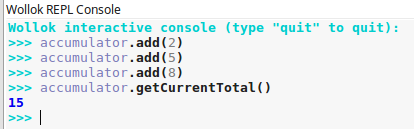
\includegraphics[scale=0.6]{../images/accumulator-repl.png}
 \caption{\small Sample usage of the accumulator object in the REPL}
 \label{fig:repl}
\end{figure}


%This is also consistent with some modern industrial OO languages that allow to define both classes or standalone objects, such as Scala \cite{Oder04a}.

%To build this first program students are not required to know about typing, scoping or packaging.
%The only required construct is the \code{program} and the only command is a message send.
%Both the receiver and the parameters are built-in objects which will be handled in the same way as user-defined objects.
%The concepts required to understand this program are no more than program, object, message and argument passing.

Shortly after in the course, we introduce unit testing which slowly replaces the REPL as the main form of interacting with objects. Figure \ref{fig:test} shows a sample test for the previous program. 

\begin{figure}[ht]
 \centering
 \begin{lstlisting}[language=Wollok]
 	import accumulator.*

	test "adding 2+5+8 should give 15" {
		accumulator.add(2)
		accumulator.add(5)
		accumulator.add(8)
		assert.equals(15, accumulator.getCurrentTotal())		
	}
   
	test "accumulator starts with 0" {
		assert.equals(0, accumulator.getCurrentTotal())
	}\end{lstlisting}
\vspace{-3mm}
\caption{\small Sample test Wollok program.}
\vspace{-5mm}
\label{fig:test}
\end{figure}

Again, Wollok is fine-tuned for our pedagogical objectives.
In particular, the test runner guarantees that there is no interaction between tests: the messages sent to the accumulator in the first test will not affect the state of the accumulator in the second test\np{sería lindo tener una cita a alguna regla de unit testing que proponga esto}.
Furthermore, tests have to be written in a separate file.
However, this decision introduces a problem: the objects (and later on, classes) defined in a different file must be accesible from the test file. With this purpose, Wollok includes a simple form of the \texttt{\textbf{import}} directive, which refers to a object/class definition file in the same folder than the test file. In this way, some basic knowledge of modularization is subtly introduced early in the course\footnote{The assimilation of the \texttt{import} directive, as early as in the second week, was not problematic in our experience using Wollok for first-year programming courses.}.

%Tests have to be written in a separate file; the directive \texttt{
%\textbf{import} accumulator.*} at the beginning of the example indicates that all the objects (and later on, classes) defined in the file called \texttt{accumulator.wlk} are available to be used in the test. In this way, some basic knowledge of modularization is subtly introduced at the very beginning of the course\footnote{\carlostext{The assimilation of the \texttt{import} directive at the second week, was not problematic in our experience using Wollok for first-year programming courses.}}. 
%Furthermore, }
%For example, tests have to be written in a separate file, which introduces the student into some basic knowledge of modularization.
%Also, 
%the test runner guarantees that there is no interaction between tests: the messages sent to the accumulator in the first test will not affect the state of the accumulator in the second test\np{sería lindo tener una cita a alguna regla de unit testing que proponga esto}.

\medskip
% Misceláneos
% Profundizar y pulir el highlighting the conceptos primarios y la estratificacion de conceptos
Another simple feature that is very helpful in the initial steps of the course is the presence of literals for lists (\eg \code{[1,2,3]}) and sets (\eg \code{\#\{1,2,3\}}).
This allows us to use collections and, therefore, increase the complexity of examples that we can build before introducing classes.
We even briefly introduce \emph{closures} at the initial stage of the course.
For example, our \code{accumulator} object can be implemented as shown in Fig. \ref{fig:accumulator/list}.
%Also \emph{Collection literals} reduce boilerplate on object creation, 
%since we think that the excess of bureaucracy to create an object helps to build up 
%the belief that using objects or collections is far more complicated than using numbers or strings, which in turns leads to \emph{primitive obsession} \cite{fowler_refactoring:_1999}.

\vspace{-3mm}
\begin{figure}[ht]
 \centering
 \begin{lstlisting}[language=Wollok]
	object listBasedAccumulator {
		var history = []
		
		method getCurrentTotal() {
			return history.sum()
		}
		method add(amount) { history.add(amount) }
		method evenCount() {
		  return history.count({n => n % 2 == 0})
		}
	}\end{lstlisting}
\vspace{-3mm}
 \caption{\small Another accumulator implementation, using a list.}
\vspace{-3mm}
 \label{fig:accumulator/list}
\end{figure}

\medskip
Next in the course, we introduce classes.
Once more, Wollok helps us in the transition: any pre-existent stand-alone object can be converted into a class by just changing the keyword \code{object} for \code{class}\footnote{As a matter of fact, we will also change the name, as our code convention mandates lowercase names for objects and uppercase names for classes}, as shown in Fig. \ref{fig:accumulator/classes}.

\begin{figure}[ht]
 \centering
 \begin{lstlisting}[language=Wollok]
	class ListBasedAccumulator {
		var history = []
		
		method getCurrentTotal() { 
			return history.sum() 
		}
		method add(amount) { history.add(amount) }
		method evenCount() { 
		  return history.count({n => n % 2 == 0})
		}
	}\end{lstlisting}
\vspace{-3mm}
\caption{\small A third accumulator implementation, class based.}
\label{fig:accumulator/classes}
\end{figure}

Figure \ref{fig:polymorphism} shows how the three previous definitions of accumulator can be used polymorphically. 
\cl{la siguiente frase, incluyendo el footnote, es reemplazada por el texto que propongo agregar al introducir colecciones.}
Also, it shows the usage of more advanced list messages and closures\footnote{In our approach, we introduce polymorphism and closures \emph{before} classes. For reasons of space we skipped those intermediate examples here.}.
A special mention has to be made about the fact that stand-alone objects are used in the same program and even they are polymorphic with class-based objects.

\begin{figure}[ht]
\vspace{-3mm}
 \centering
 \begin{lstlisting}[language=Wollok]
 	import accumulator.*

	test "adding 2+5+8 should give 15" {
		const accumulators = [ 
			accumulator, 
			listBasedAccumulator,
			new ListBasedAccumulator()
		]

		accumulators.forEach { accum =>
			accum.add(2)
			accum.add(5)
			accum.add(8)
			assert.equals(15, accum.getCurrentTotal())	
		}
	}\end{lstlisting}
\vspace{-3mm}
\caption{\small Simple polymorphism example.}
\label{fig:polymorphism}
\end{figure}

% Effect
Finally, Wollok includes features that allow for discussing about \emph{controlling side effects} in an early stage of programming courses, making programmers aware of the potential side effects of each portion of code.
The most basic of these features is the ability to 
differentiate variables from constants (defined using \code{var} and \code{const} resp.).
Moreover, methods not including a \texttt{return} expression are considered as \emph{void}, \ie\ they do not yield a value and no operation can be applied to them. Furthermore, the REPL does not show any text as result of the evaluation of void methods, as can be seen in Fig.~\ref{fig:repl}.

\section{A Customized Programming Environment}
\label{sec:environment}

The features that influence the experience of the learning programmer are not limited to the programming language used. 
The \emph{tools} used to write, analyse and evaluate the code have a paramount relevance for this experience, and therefore for the success of the programming courses.

Beginner programmers are likely to require more guidance and make more mistakes than experienced ones.
Also, the kind of support required by a experienced programmer from her development environment is different from that required by a beginner, \eg an experienced programmer might select her programming environment thinking on increasing productivity.
One very important feature a beginner requires from her programming environment is \emph{discoverability}, \ie the tools should help discover possible paths of action and gently provide feedback when the student makes a mistake, helping her to understand what was wrong and how to fix the program.
Finally, all programmers require tools that help them understand, navigate and explore their programs.

We decided to embed the Wollok language in an integrated programming environment, whose features are designed having in mind the specific needs of novice programmers.
In our view. the tools provided by the environment are a fundamental part of the Wollok proposal, in equal terms with the language features.
In particular, the Wollok environment provides tools focused to the following goals:
\begin{itemize}
\item To guide and ease the actual code writing.
\item To detect several of the most common mistakes done by novices, providing adequate feedback, and even to provide possible corrections whenever is possible.
\item To navigate and give different perspectives of the defined objects and classes.
\item To test and experiment with objects, both those provided by the student and those provided by Wollok.
\end{itemize}

	We remark that several of the tools that the Wollok environment provides are common, in exact or approximate form, to those provided by mainstream industrial IDEs like Eclipse, Visual Studio or the Idea series. In this way, we aim to make both the programming experience more appealing to the students, and the transition to later courses and work environments softer; while giving adequate support to the learning process through the same tools.



%%%%%%%%%%%%%%%%%%%%%%%%%%%%%%%%%%
\subsection{Basic guidance for writing code}
We have noticed that the syntactic strictness of programming languages imposes a harsh barrier on novice programmers. 
Errors due to mispelled keywords or lack of proper delimiter (brace/bracket/parenthesis) match are both frequent and frustrating to them\footnote{Of course, block-based and visual programming tools make these problems just vanish. As we describe in the discussion, such tools would not be adequate for the intended uses of Wollok.}.
The Wollok IDE code editor offers several basic features that help to mitigate such frustrations. We mention syntax highlighting, automatic insertion of the closing delimiter when the opening one is typed, and the proposal of a proper indentation scheme. We remark that the latter feature also aims to improve readability of code, and also to induce good code organization practices.

The Wollok IDE also provides \emph{content assist}, 
\ie in certain contexts, the IDE can autocomplete an identifier name or provide a list of possible completions if there are many (\cf Fig. \ref{fig:codeCompletion}).
This is available for all types of variables, constants and messages sent to \code{self}, \code{super} or any WKO\footnote{Extending autocomplete to every message send is a difficult task, due to the lack of explicit type information. 
Current work in progress includes a \emph{type inferer} that will improve the content assistance capabilities of Wollok.}. 
 
\begin{figure}[ht]
 \centering
 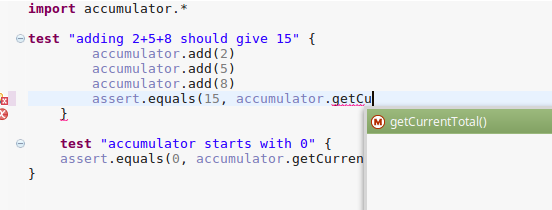
\includegraphics[scale=0.45]{images/codeCompletion.png}
 \caption{\small A list of suggestions from the Wollok IDE content assistance.}
 \label{fig:codeCompletion}
\end{figure}

At a bigger scale, Wollok admits the definition of several objects and/or classes in the same file. 
This allows the teacher to go deeper in the initial examples using several objects and polymorphism without requiring the students to struggle with imports and packages.
These concepts will arise later in the course, when students' programs increase their complexity to a level that demands for modularization. 
%(\cf \ref{sec:modularization}).


%% To guide and ease the acual code writing
%We have noticed that the first barrier for novices is the strictness of a programming language syntax. Frequently initial students find annoying that their program will not execute if they forget a closing brace or mispell a keyword or a variable name, in many cases even a case error stops execution or produces unexpected results.
%Syntax highlighting is very helpful by providing a very fast visual feedback about a mispelled keyword.
%Also, like many modern code editors, the Wollok IDE automatically creates a matching closing symbol each time the programmer types a parenthesis, square bracket or brace. 
%Also the IDE helps correctly indenting the code inside code portions enclosed in braces or square brackets, which both helps avoiding frustrating syntax problems and starts to induce best practices about code organization.
%
%Other approaches have addressed this problem using block-based or visual programming tools \np{Cita a alguno}. 
%While we value those ideas, we think that mainstream programming is and will continue to be text-based, therefore, non-textual programming can be useful for younger students, but at universitary level it is better to provide tools that help dealing with syntax problems rather than continue circumventing them.
%
%At a bigger scale, Wollok admits the definition of several objects and/or classes in the same file. 
%Allowing the teacher to go deeper in the initial examples using several objects and polymorphism, without requiring the students to struggle with imports and packages.
%These concepts will arise later in the course, when students' programs increase their complexity to a level that demands for modularization. 
%%(\cf \ref{sec:modularization}).
%\np{¿Esto no es una característica del lenguaje?}
%
%The Wollok IDE also provides \emph{content assist}, 
%\ie in certain contexts, the IDE can autocomplete an identifier name, or provide a list of possible completions if there are many (\cf Fig. \ref{fig:codeCompletion}).
%This is available for all types of variables and constants and messages sent to \code{self}, \code{super} or any WKO\footnote{Current work in progress includes a type inference system that once completed should allow to add content asistance for any message send}. 
 %
%\begin{figure}[ht]
 %\centering
 %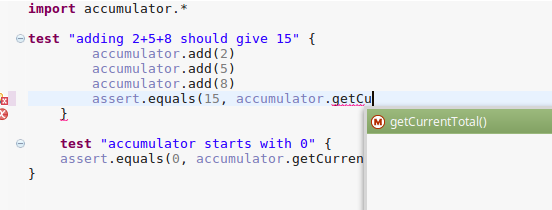
\includegraphics[scale=0.45]{images/codeCompletion.png}
 %\caption{\small A list of suggestions from the Wollok IDE content assistance.}
 %\label{fig:codeCompletion}
%\end{figure}
%


%%%%%%%%%%%%%%%%%%%%%%%%%%%%%%%%%%
\subsection{Detect mistakes and help fixing them}
\label{sec:detectMistakes}
The Wollok IDE is able to detect statically (i.e. prior to evaluation) several mistakes frequently made by students. Apart from basic errors like non-matching delimiters, mispelled keywords and references to undefined identifiers, the code analysis performed by Wollok verifies the following:
\begin{enumerate}
\item 
Class definitions must follow a definite order: instance variable declarations, followed by constructors, followed by methods. This aims to promote good code organization practices in students.
\item 
Unused or never-assigned variables are indicated as warnings. The ability to separate warnings from errors opens the way to add more checks of possible bad smells in student code.
\item 
Similarly, a variable read just once is marked as a warning, since it could be inlined.
\item 
Some cases of type error related to message sends are detected. This includes all self-sends and messages sent to WKOs.
\item 
Some subtler mistakes are also detected, e.g. a method must return in either all execution branches or none, an abstract class cannot be instantiated.
\end{enumerate}

These errors are, in fact, detected while the student is typing a program and are shown in the editor. Like in several modern code editors, the source line is marked with an error sign. When the student passes the mouse pointer over that sign, an explanatory message is shown.
Special care has been put in the messages, to explain mistakes in the same terms in which the teacher talks to students.
Finally, in some situations, the IDE proposes possible \emph{automatic fixes} to the detected problems.

Figure \ref{fig:errorReporting} exemplifies this feature along with the rendering of a code error. The mispelled identifier is underlined and if we pass over the mouse on the error report, we get an error message together with possible fix.
In this case, the automatic fix will insert an empty method in the adecquate position. 

\begin{figure}[ht]
 \centering
 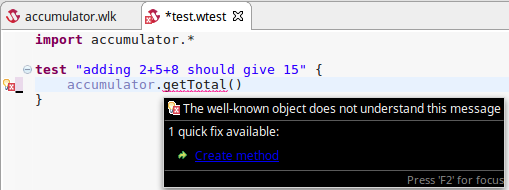
\includegraphics[scale=0.5, trim={0 0 0.15cm 0},clip]{images/errorReporting.png}
 \caption{\small Example of a simple error detection.}
 \label{fig:errorReporting}
\end{figure}

These features aim to give a quick visualization and a proper understanding of coding mistakes. In this way, we intend to empower students to explore different ideas, providing positive feedback in case of mistakes.
While this does not replace the more personalized feedback a teacher provides, in several situations, a sensitive automatic feedback helps students not to stay stuck with simple errors waiting for teacher or colleague assistance.
This, in turn, allows for more agile lab classes and, therefore, for the possibility of including more exercises during a course.

\medskip
We note that automatic detection acts as a (basic) assistant teacher, \ie some simple topics that are not crucial for the course can be left for the student to learn by herself in the interaction with the IDE, instead of to being explained in class.
This is specially useful for some errors that only some students are likely to make.
Tackling these errors in class would imply to show a bad solution to the rest of the students, who had otherwise not thought about it. While anticipating errors could be a fine strategy in an advanced course, it mostly confuse beginners.
Therefore, we prefer to let the IDE detect the mistake and show possible solutions, only for the students that effectively incur in this kind of errors.\np{Faltaría un ejemplo.}



%Another dimension of the programming environment is helping the programmer to recover from his mistakes. 
%
%First, we aim for \emph{static error detection} whenever possible, because it provides faster feedback than runtime checks.
%Some errors can be even reported as the programmer is typing.
%On the other hand, runtime checks are not only slower but also open to be skipped in some program executions.
%
%Second, error reporting should provide with clear messages, explained in the same terms in which the teacher talks to the students. 
%Also, inline error reports, \eg underlining the offending code, relieves the student from the task of mapping the detected problem with the possible cause 
%
%Third, in some situations, the IDE can propose possible automatic fixes to the detected problems.
%Figure \ref{fig:errorReporting} exemplifies these features. The mispelled identifier is underlined and if we put the mouse on the error report we get an error message and a possible fix.
%In this case, the automatic fix will insert an empty method in the adecquate position.
%
%\begin{figure}[ht]
 %\centering
 %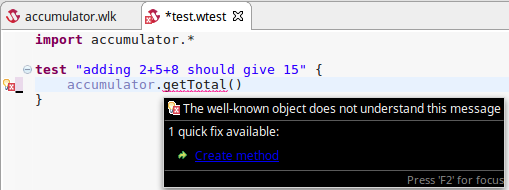
\includegraphics[scale=0.5, trim={0 0 0.15cm 0},clip]{images/errorReporting.png}
 %\caption{\small Example of a simple error detection.}
 %\label{fig:errorReporting}
%\end{figure}
%
%\medskip
%Together, these characteristics are meant to empower the student to explore different ideas, 
%providing positive feedback in case he makes a mistake.
%
%While this does not replace the more personalized feedback a teacher  provides, in several situations a sensitive automatic feedback helps the student not to stay stuck with simple errors waiting for a response.
%This in turn allows for more exercises during the course.
%
%Moreover, automatic detection acts as a (basic) assistant teacher, \ie some simple topics that are not crucial for the course can be left for the student to learn by herself in the interaction with the IDE.
%This is specially efficient for some kind of errors that occur only for specific groups of students, \eg those with previous non-academic OO experience. 
%Tackling this errors in class, would imply to show a bad solution to the rest of the students, that had otherwise not thought about it. This would be a fine strategy in an advanced course, but will confuse beginners.
%Instead, we prefer let the IDE detect the mistake and show possible solutions, only for the students that effectively incurr in these kind of errors.\np{Faltaría un ejemplo.}
%
%\medskip
%
%%  - Error indications with adequate messages. De esto daría algunos ejemplos que nos parezca piola resaltar, no sería exhaustivo.
%%  - Quick fixes.
%
%Finally, the great majority of validations and automatic proposals, are the result of our experience in the classroom, looking at the students using the Wollok language and IDE, as well as other languages and tools we have used in the past.
%Each semester, we receive reports of the teachers using Wollok which include the type of errors the students make most often, trying to improve the network of validations and proposals, in order to improve the learning experience.
%
%%\medskip
%%This validations are organized and shown in a unified way, using a dedicated section of the user interface for their display.
%%All the results of the checking and the validation of the program is shown in one integrated view, it is called \emph{Problems View}, Fig. \figref{problemsview.png} shows a view of this feature. 
%%
%%\begin{figure}[ht]
%%    \centering
%%	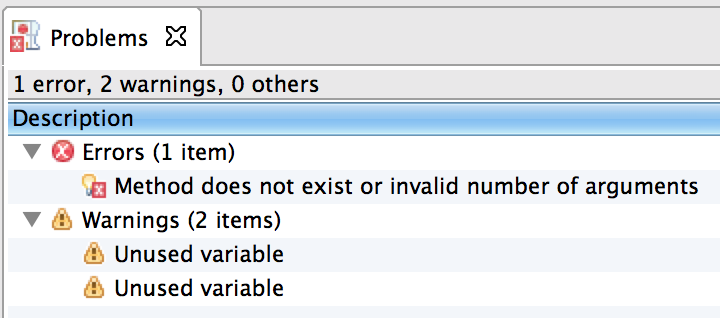
\includegraphics[scale=0.5]{images/wollok-paper-check-problemsview.png}
%%    \caption{Problems View: shows the different problems detected by the IDE }
%%    \label{fig:problemsview.png}
%%\end{figure}
%%
%%Here is a list of all the validations and checks the tool supports, and a brief reason why they are useful while teaching object oriented programming:
%
%%  \item \textbf{References resolution problems}: this errors are useful to detect and avoid references to undeclared variables and also errors in the sending of messages.
%%	\begin{itemize}
%%	  \item \textit{Undeclared references}: from local variables, parameters or internal fields of objects and classes.
%%	  \item \textit{Undefined constructors}: checking for the number and type of the parameters.
%%	  \item \textit{Messages to this}: sending messages to this is a special case, here we can check the existence of the correct method by the number and type of the arguments, even without using type inference.



%%%%%%%%%%%%%%%%%%%%%%%%%%%%%%%%%%
\subsection{Understanding and navigating a program}
Code navigation and visualization tools can significantly improve the programming experience.
We note that in our teaching (and also industrial) experience, lack of such tools might mislead students (resp. developers) to avoid correct modularization of their program, as they run into difficulties coping with a program that is divided in several small pieces.

The Wollok IDE offers several keyboard/mouse shortcuts for code navigation, allowing e.g. to jump from a class reference (tipically, for instance creation) to its definition, from a message send to the corresponding method (when such method can be determined) and back-and-forth navigation on code portions resembling that of Web browsers.
These tools allow for a better understanding of the relationship between the different portions of the code being developed by a student.

Some code visualization tools are available as well. An outline view and automatically generated static diagrams (\cf Fig. \ref{fig:outline} right and left resp.) provide streamlined views of the classes and WKOs defined. Clicking a class, WKO or method pops up the corresponding definition in the code editor.
We claim that these tools are particularly useful to induce students to abstract themselves from the details of some portions of a program, understanding objects and classes as black boxes that provide some services, instead of attempting to have all of them in their head at all times. This level of abstraction is a necessary skill for being able to participate in larger projects.

\begin{figure}[ht]
 \centering
 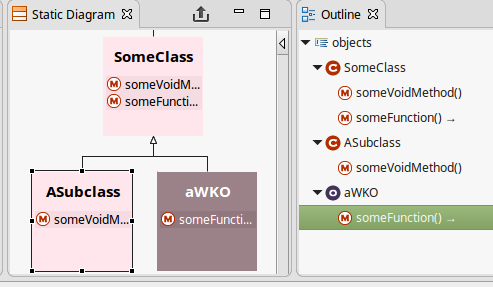
\includegraphics[scale=0.5]{images/outline.png}
 \caption{\small Static diagram and outline.}
 \label{fig:outline}
\end{figure}

The Wollok IDE also includes some tools to help students to manage the whole set of code produced along a course.
Source files are organized in \emph{projects}, which have a predefined directory structure including both files for class/object definitions and tests.
The generated file structure is adequate to the use of a source code repository such as GIT or SVN.
These features alleviate the frequent difficulties novice programmers find to organize their source files and, in particular, to coordinate work in group assignments.
We note to this respect that it is normal to see members of a work group sharing code by sending e-mail with \emph{zip files} between each other.
The time spent trying to reconcile different versions of the program, or even trying to understand which is the latest one, distracts them from learning the actual topics of the course.
Another benefit of providing suitable source organization tools is the enforcement of good development practices.

%At a higher level, the Wollok IDE is designed to help the students to put in order the code they produce along the course. 
%Source files are organized in \emph{projects}, that have a predefined directory structure including both files for class/object definitions and tests.
%The generated file structure is adequate to the use of a source code repository such as GIT or SVN, improving collaboration in group assignments and serving as a communication tool with teachers.
%%Frequently this is also accompanied by a source code repository such as GIT or SVN, which not only helps organization but also improves collaboration in group assignments and serves as communication tool with the teacher.
%
%These features solve the frequent difficulties novice programmers find to organize their source files, and in particular, to coordinate work in group assignments.
%We note to this respect that it is normal to see members of a work group sharing code by sending e-mail with \emph{zip files} between each other.
%The time spent trying to reconcile different versions of the program or even trying to understand which is the latest one, distracts them from learning the actual topics of the course.
%Hence the benefit of providing suitable source organization tools, besides the promotion of good development practices it implies.


%Simple \emph{code navigation} tools can significantly improve the programming experience.
%For example the Wollok IDE allows to go in one click from a message send to its implementation\footnote{In the cases that is identifiable by the static analyser} and a keyboard shortcut\footnote{\code{ALT + left arrow} which is familiar to students due to its universal adoption in web browsers.} to go back to the previous location.
%Fast navigation back and forth through a program allows for better understanding of the relationship between the different portions of it.
%We have seen that lack of proper navigation tools might mislead the student to avoid correct modularization of their program, as they run into difficulties coping with a program that is divided in several small pieces.
%
%Also, code visualization tools help understanding bigger programs and are as useful for beginners as they are for experienced programmers.
%The Wollok IDE provides an outline view and automatic static diagrams (\cf Fig. \ref{fig:outline}).
%These higher-level views of the program, allow the student to gain practice in abstracting herself of the details of some portions of a program, understanding her objects and classes as black boxes that provide some services, instead of attempting to have all of them in her head at all times. This level of abstraction is a necessary skill for being able to participate in a larger project.
%
%\begin{figure}[ht]
 %\centering
 %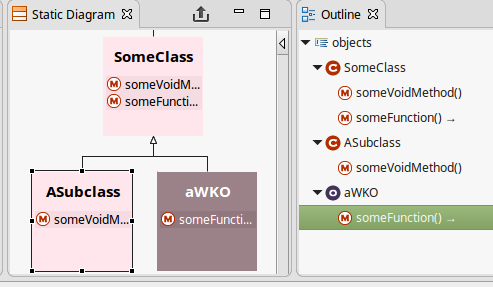
\includegraphics[scale=0.5]{images/outline.png}
 %\caption{\small Static diagram and outline.}
 %\label{fig:outline}
%\end{figure}
%
%% No puse nada de:
%% - Ctrl-O, es medio difícil de explicar, no sé.
%% - Tampoco sé bien bien qué decir del Ctrl-E
%% - Destacar que distingue los métodos con y sin efecto, si bien esto es un feature interesante, creo que es medio descolgado en este punto o habría que hablar más largo sobre por qué esa diferenciación que no está en ningún lado, creo.


%%%%%%%%%%%%%%%%%%%%%%%%%%%%%%%%%%
%\subsection{Encouraging best programming practices}
%In our opinion, good practics should be taught from the very beginning of programming curricula. This claim is independent of the recurrent debate about rules and conventions. 
%Our experience shows that it is unlikely that novice programmers appreciate the advantages of e.g. good variable names or correct code indentation, as these attributes are more easily appreciated on larger programs.
%Therefore, we have to actively enforce them, and get them used to writing and reading good quality code.
%
%Several features of the language and code editor aim to promote, or enforce, good programming practices.
%For example, it compels the programmer to a predefined order inside a class definition, \ie grouping all variables and constants in the first place, then constructors and finally methods. 
%Also it establishes some basic rules about naming and restricts the usage of global variables.
%We also mention that autocompletion of braces and square brackets eases the adoption of adequate indentation.
%
%Moreover, some bad programming habits are detected by the error detection of the IDE. 
%As an example, Fig. \figref{check-unusedVariable} shows an example of an unused variable error.
%Unused, \emph{dead code} tends to appear after a refactoring or after trying different solutions to a problem. 
%Quick detection of this kind of errors will help the student to identify the bad practice and train her to avoid its appearance.
%
%
%\commented{
%A major part of the IDE is devoted to enforce good programming practices, which we consider as a main topic in a programming learning course.
%For example, it compels the programmer to a predefined order inside a class definition, \ie grouping all variables and constants in the first place, then constructors and finally methods. 
%Also it establishes some basic rules about naming and restricts the usage of global variables.
%
%While the specific rules could be debated forever, and independently of the conventions chosen,
%we think that good programming practices have to be taught from the very beginning.
%In their first programs, students might not be able to appreciate the advantages of good variable names or correct code indentation, these are attributes that are more easily appreciated on larger programs.
%Therefore, we have to actively enforce them, and have them get used to writing and reading good quality code.
%We do not want them to acquire bad programming practices that will be difficult to \emph{unlearn} later.
%
%As an example, Fig. \figref{check-unusedVariable.png} shows an example of an unused variable error.
%Unused, \emph{dead code} tends to appear after a refactoring or after trying different solutions to a problem. 
%Quick detection of this kind of errors will help the student to identify the bad practice and train her avoiding its appearance.
%}
%
%\begin{figure}[ht]
    %\centering
	%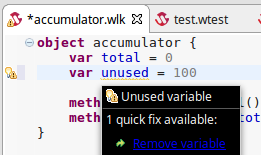
\includegraphics[scale=0.6]{images/wollok-paper-check-unusedVariable.png}
    %\caption{Detection of unused variables}
    %\label{fig:check-unusedVariable}
%\end{figure}
%
%\medskip
%At a higher level, the Wollok IDE is designed to help the students to put in order the code they produce along the course. 
%Source files are organized in \emph{projects}, that have a predefined directory structure including both files for class/object definitions and tests.
%The generated file structure is adequate to the use of a source code repository such as GIT or SVN, improving collaboration in group assignments and serving as a communication tool with teachers.
%%Frequently this is also accompanied by a source code repository such as GIT or SVN, which not only helps organization but also improves collaboration in group assignments and serves as communication tool with the teacher.
%
%These features solve the frequent difficulties novice programmers find to organize their source files, and in particular, to coordinate work in group assignments.
%We note to this respect that it is normal to see members of a work group sharing code by sending e-mail with \emph{zip files} between each other.
%The time spent trying to reconcile different versions of the program or even trying to understand which is the latest one, distracts them from learning the actual topics of the course.
%Hence the benefit of providing suitable source organization tools, besides the promotion of good development practices it implies.
%
%%We note that without adequate IDE support, the organization of source files often pose difficulties to novice programmers. In particular, the coordination of work for group assignments can be problematic. 
%%For example, 
%%%in the absence of adequate tools 
%%it is ordinary to see members of a work group share code by sending \emph{zips} by e-mail between each other.
%%The time spent trying to reconcile different versions of the program or even trying to understand which is the latest one, distracts them from learning the actual topics of the course.
%%
%%Without adequate guidance, a group of novices, who have yet not assimilated an autonomous organization discipline, will usually encounter difficulties structuring their code or coordinating their work.
%%For example, in the absence of better tools it is ordinary to see members of a work group share code by sending \emph{zips} by e-mail between each other.
%%The time spent trying to reconcile different versions of the program or even trying to understand which is the latest one, distracts them from learning the actual topics of the course.



%%%%%%%%%%%%%%%%%%%%%%%%%%%%%%%%%%
\subsection{Tests and experiments}
As we described in Section \ref{sec:wollokLanguage}, Wollok provides two ways of working with the defined objects and classes: the REPL and the definition of tests.

The REPL provides a simple environment for direct object manipulation; it is the first tool to interact with objects that we introduce in the course.
The programmer can just send messages to the WKOs she defines and see how they respond. 
In some courses, we even \emph{start} on the REPL by sending messages to objects provided by the teacher.
In this way, students get familiarized with the most important concepts of the OO paradigm: \emph{object} and \emph{message}, before going into the details about how these objects have been implemented.
Moreover, the REPL also allows the programmer to define local variables, which are useful to remember intermediate results to be used in further operations, making it easy for the students to perform non-trivial object manipulations.

\medskip
As the REPL interaction grows, in a short time the students themselves realize that they are doing repetitive operations there and start looking for automation;
at this moment, \emph{automatic tests} are introduced.
Fig. \ref{fig:testRunner.png} shows the test runner tool output for the test shown in Fig. \ref{fig:test}.

It is important to notice that the test requires a \emph{higher level of abstraction} than the REPL.
Now the student has to anticipate the result that some expression should yield. Writing explicitly both the expression and the expected result, and interpreting a \emph{green bar} as a signal that the answer yielded was the expected, without ever seeing it.

We observe that, once the students become more fluent with automated tests, they use the REPL with less frequence, even while it is available all along the course.
Also, we remark that by the combination of REPL and tests, we have succeeded in completely avoiding the need for undesired debugging practices, such as the inclusion of \code{println} expressions along the code.

\begin{figure}[ht]
    \centering
	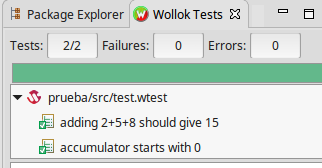
\includegraphics[scale=0.6]{images/testRunner.png}
    \caption{Test runner view after a sucessful test run.}
    \label{fig:testRunner.png}
\vspace{-5mm}
\end{figure}

%\subsection{Type Inference}
% Type inferer
%Another distinctive characteristic of the Wollok project is the type inferer.
%We think that type inference is key to a simple programming environment.
%On one side, it allows to detect lots of common mistakes \emph{before running the program}:
%if an object does understand a message, if a wrong argument is passed, if incompatible types are mixed or even miss-spellings.
%In environments without this capability it takes more time to detect errors.
%Moreover, it is not uncommon that a type mistake produces a runtime error in a place different from where the mistake was done, producing confusion.
%
%Still, providing a type inferer for a language such as Wollok has many subtleties, which deserves an independent study \cite{passerini_nicolas_extensible_2014}.
%On one side we require it to be able to work without type annotations and at the same time provide feedback useful for an inexperienced programmer.
%On the other side, the type system is rather complex;
%for example, the presence of stand-alone objects requires the type system to handle \emph{structural types}, since a named type system would not allow them to be treated polymorphically.
%Also, we want to be able to treat polymorphically stand alone objects with class-based objects.
%\figref{check-messageSending.png} shows an error detected by the type inferer and how it shows the information to the programmer.
%Notice that the inferred type for the object \code{ufo} is a structural type: \code{fly}
%
%\begin{figure}[ht]
%    \centering
%	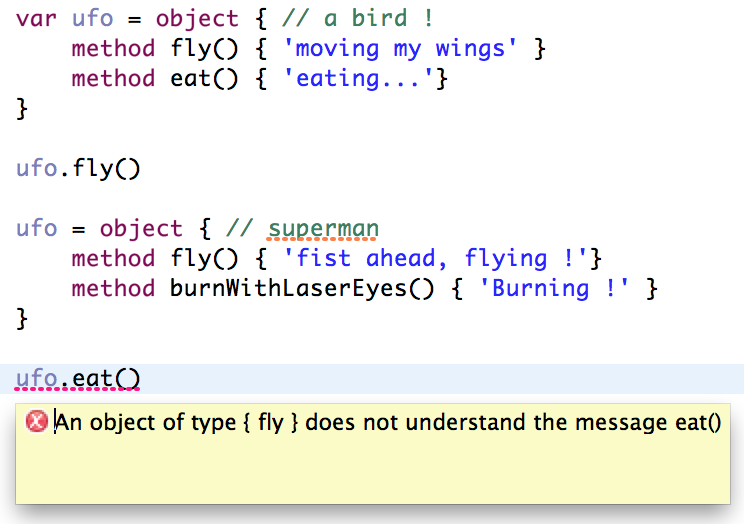
\includegraphics[scale=0.5]{images/wollok-paper-check-messageSending.png}
%    \caption{Type system in action, detecting not defined method for the message sent}
%    \label{fig:check-messageSending.png}
%\end{figure}
%
%

%\subsection{Implementation}
\label{sec:implementation}

The way wollok is implemented is essential to enable us to build a fully customized educational language with a industrial-level toolset.
After many years of experience in the Ozono project and its predecessor, we arrived to the conclussion that
the limitations of a language implemented as an embedded DSL \cite{Mern05a} produce hindrances in the learning process (\cf Sec. \ref{sec:newLanguage}).
Still, giving up the embedded implementation strategy is not conceivable if we have to create all the required tools "from scratch".
Also we require a flexible implementation that allows the language to evolve, enabling and supporting our research activities.

The current implementation of Wollok language is built on top of Xtext\footnote{\url{http://www.eclipse.org/Xtext/}}, 
which is an Eclipse\footnote{\url{https://www.eclipse.org/home/index.php}}-based Language Workbench\cite{fowler2005language}.
By providing a set of tools for language development, the Xtext workbench allows us to get rid of some the necessary effort required to build a language and IDE.
Out from the language grammar, which is defined as an extended BNF, the workbench provides several parts of the infrastructure a language requires: 
a parser, an object-oriented AST representation\footnote{The AST is represented as Java ECore models, which are part of the EMF project \url{http://www.eclipse.org/modeling/emf}}, 
an editor capable of syntax and error highlighting, basic content-assist (\cf \figref{codetemplates.png}) and cross-references search, 
and other tools attached to the IDE, such as structured views of the code (\cf \figref{outline.png}).
Also, it gives us support for implementing more advanced tools such as quick-fixes, refactorings and UI Wizards for creating projects other Wollok entities.
The IDE is integrated into the Eclipse platform, which in turn also helped us integrating with other Eclipse tools, such as the JUnit test runner and a debugger.

\begin{figure}[ht]
    \centering
	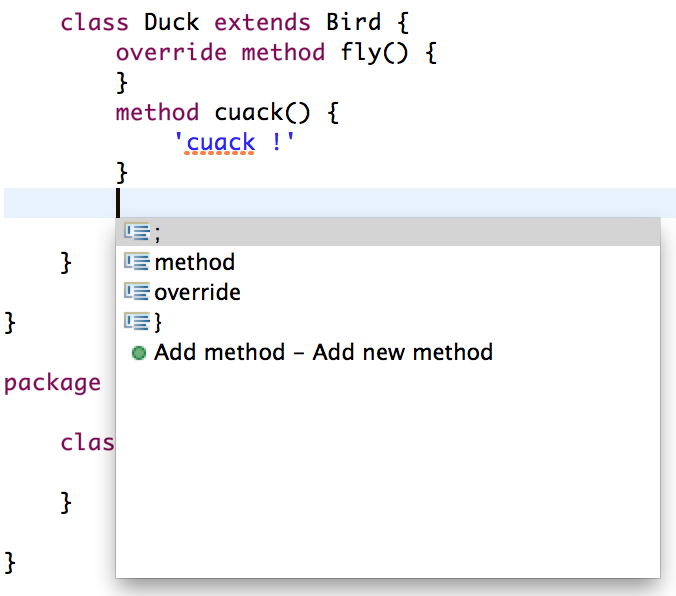
\includegraphics[scale=0.5]{images/wollok-paper-codetemplates.png}
    \caption{Code Assist: code templates for easy edition}
    \label{fig:codetemplates.png}
\end{figure}

\begin{figure}[ht]
    \centering
	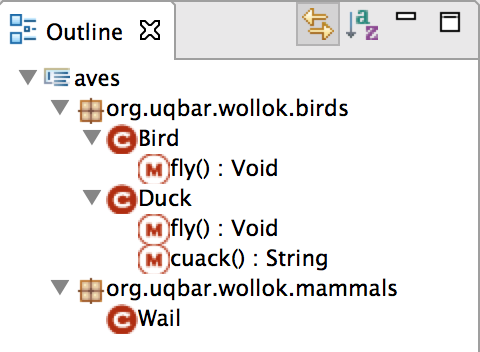
\includegraphics[scale=0.5]{images/wollok-paper-outline.png}
    \caption{Outline View: This view shows the structure of the file.}
    \label{fig:outline.png}
\end{figure}

% Interpreter
Wollok is implemented as a fully interpreted language, implemented as a Java application. 
The other standard XText implementation strategies involve generating Java code, which is very difficult to achieve out of a language without a single type annotation.
The downside of this decision is that we lost the \emph{out-of-the-box} type-checked code generation provided by XText, together with the XText standard debugger.

Regarding the debugger, we developed a custom eclipse plugin which already provides a good portion of the features provided by many industrial type language debuggers.
This debugger can even be abstracted into a reusable XText component for any other interpreted language.

% \subsection{Type System}
% XText type system is currently implemented on top of XSemantics\footnote{http://xsemantics.sourceforge.net}, a DSL for writing rules for XText languages. XSemantics is itself made with XText.
% This allows us to develop our type system in a declarative way. The type system can be seen in action in \figref{check-messageSending.png}.

\medskip
% \subsection{Development}
To allow for a graceful evolution of the language and the development environment, we also had to tailor our development practices.
While these ideas are not novel in indutrial developments, usually they do not have a lot of consideration in research projects or language development projects,
and a good bit of effort is required to adapt common industrial techniques to the specific needs of our project.

On one hand, we have been emphatic on the necessity for automated unit testing.
As said before, the difficulties which arise in testing a language implementation are quite challenging and different from other kinds of software.
Wollok combines several techniques for testing its development.
Part of the interpreter logic is being tested with unit tests in JUnit, 
while for the aspects that are more tied up with XText and Eclipse components we are using XPect\footnote{\url{http://www.xpect-tests.org}}, 
a unit and integration-testing framework for Xtext languages.
XPect is in turn also developed as an XText language.
It provides a declarative way to annotate Wollok programs with expected behaviour like validator’s errors/warnings, or code completions, etc.

On the othe hand, the deployment and distribution of Wollok is fully automated.
Combining several tools such as Github, Maven, Tycho, Travis CI, and Eclipse update sites we generated an infrastructure in which new versions can be released just with a pull request.
We have two distribution strategies: as a standalone product or as a plugin that can be added into any Eclipse instance.
Taking advantage of the Eclipse update sites, we allow the students to update their IDE without requiring a new installation.
This, in turn, allows us for a very fast development cycle for resolving potential errors or critical changes.
Finally, we distribute both \emph{stable} and \emph{development} versions. 
While the former are best for students, the latter are interesting for teachers which desire to get a glance of the new features in advance.

\section{Classroom Experience with wollok}
\label{sec:experience}

% Lo simple que les resulto a los chicos trabajar con una IDE
Let us describe the first experience of a new student with Wollok.
At the very beginning, the student starts by interacting with just two windows: the code editor, which points to an initial source file, and the REPL.
All the coding is done inside the editor, which includes the features of highlighting, autocompletion and error detection/correction we described in Section \ref{sec:detectMistakes}. 
The streamlined WKO syntax of Wollok allows for defining simple objects with a minimum of elements. 
A menu option gives access to the REPL, where the defined WKOs can be accesed by their global names so that it is straightforward to interact with them. 
In the interaction through the REPL, void methods are easily distinguished from those returning a value. 
Furthermore, typing just an object name results in a simplified internal view that displays the attributes along with their values.

Further on, the language and IDE features permit a gentle introduction to each successive concept we work with in the course. 
In particular, the absence of explicit type information allows for a simple implementation of polymorphism between WKOs: it suffices to have different objects that define methods for the same message.
We also remark the similarity of the syntax for WKOs and classes, described in \secref{wollokLanguage}, 
consent a smooth transition to the latter, motivated by the natural desire of having multiple object that share the same definition, having at the same time separate states.

While introducing design patterns is not a part of the initial OOP subject, we observe that some patterns appear naturally as we evolve to more complex problem statements.
For example the idea of Singleton is natural in Wollok as classes and globally accesible WKOs can be combined in the same program. 
Moreover, short class/object definitions can be easily added to an existing Wollok program, leading to the creation of little objects that provide specific behaviours. 
We note that the features of Wollok favor the reification of concepts that are not linked with the state that has to be modeled or handled. 
Sometimes the resulting objects follow, e.g., the Strategy or State~\cite{Gamm93b} patterns.


\section{Discussion}
\label{sec:discussion}

% Discussion of actual solution \emph{vs.} initial constraints from \ref{sec:problem}. Explain the space of the solution, why we made it this way.
% Evaluation of the solution. How does the solution meet the criteria? Where does it succeed or fails...

\subsection{A brand new language}
\label{sec:newLanguage}
% Hacer o no hacer un lenguaje nuevo.
A common point of controversy is whether is is worth to create a brand new language and toolset, 
instead of building our pedagogical ideas on top of existing ones, such as Self, Ruby, Smalltalk or even Eiffel.
In our experience, begginning programmers require different features from their working environment that advanced programmers
and the right selection of tools and concepts can produce substantial improvements in the learning process.
Therefore, we believe that the possibility of fine tuning provided by a specialized environment largely pays for the additional effort.

Each semester, a group of more than 20 teachers in 3 different universities share their experience with the language and tools and discuss about new features and changes to the system. 
Every modification is guided by a shared understanding about how to teach OOP \cite{lombardi_instances_2007,lombardi_carlos_alumnos_2008,griggio_programming_2011,spigariol_lucas_ensenando_2013}
% y que muestran las grandes posibilidades que se dan a partir de esta decisión inicial: imports, tests y manejo de propiedades.

A good example about teaching-specific language-design decisions is Wollok import system,
\ie the way that a programming language allows the programmer to refer in one unit of code (for example a file) to program entities defined elsewhere.
The import system allows the student to write his first very simple programs without knowing about packages or modularization, which are far too complex for him at the beginning. Still, later in the course modularization concepts are introduced and even the language forces the student to separate his code in different units. 
A full description of how the import system works and other syntax decisions can be found in \cite{javier_fernandes_wollok_2014}.

\subsection{To IDE or not to IDE}
Another frequent controversy between software programmers is about the convenience of using an IDE or a simpler text editor for writing code. In the last decade, several languages, frameworks and other tools have became popular for which there are fewer visual or integrated environments. 

This scarcity of tools has diverse roots. In some cases, the lack of type information undermines the possibility to implement features such as code completion, automatic refactorings or code navigation.
In other cases the velocity of change in languages and frameworks makes it impossible for the tools to catch up.
Frequently there is also a matter of taste, some (maybe younger) developers prefer lighter programming environments.
In the teaching environment, it has been claimed that providing the student with too much tools will make them dependent of those tools.

In our view, tools that simplify day to day work can not be neglected. We recognize that the availability of tools for several modern tecnologies is limited, but still we see that professional programmers make use of a good amount of tools to program consistently and efficiently.
Proof of this is that the most popular text editors in industry are those that allow for additions in the form of plugins, where the programmer can create his own personalized development environment.
Other tools that are not integrated into the development environment, are inserted into the development process by other means; for example a continuous integration process may run a \emph{linter} on each commit, check the build and run tests.

So, instead of a discussion about whether we need powerful tools, we rather see an evolution from heavy monolithic environments with lots of tools onto an ecosystem of light tools that have different ways to integrate with each other allowing a developer or team to create a unique environment which accomodates to their specific needs and taste. 

Still, in our specific case, we opted for an \emph{integrated} environment, because it simplifies the set up for beginners as they only have to install one piece of software which comes with all the tools they will need for the course. In more advanced courses, we think that it could be a good idea to let the students build their own environments.

Finally, we think that teaching programming should include teaching the best practices that we see in the professional world. A student which knows the best practices and tools that are used in professional software development will have a significant advantage over those who lack these knowledge.

%\subsection{Image vs. files}
%Unlike many traditional OO programming environments, which are image-based, Wollok is file-based.
%While we have found solid grounds for taking this decission (\cf \secref{file-based}), 
%we also recognize the importance of a \emph{live object environment}, 
%\ie a work space in which the programmer can interact with live objects by sending them messages.
%As in many file-based OO and scripting languages, in Wollok this kind of interaction is achieved through an interactive console or 
%REPL\footnote{Read-eval-print-loop \cite{hey2014computing}.}
%The interactive console allows the programmer to inspect the state of his program or modify it, both at the end of an execution or in the middle of a debug session.
%However, right now we do not provide a way to modify the program while it is running, as it happens in classigal image-based environments.
%This kind of features have been postponed because we we think that modifying the code in the middle of a program run 
%usually has subtle consecuences that are difficult to grasp for an unexperienced programmer.
%It is not uncommon to see that students get confused when they try to modify live code, 
%so there is a high price to pay with little to gain in return.


%\section{Related Work}
%\label{sec:related}

% Other solutions in the domain, and a real comparison of our contribution with solutions from other people.
BlueJ \cite{bennedsen_bluej_2010} is an educative environment for programming in Java 
which shares several points of view with our approach (\cf \secref{related}).




Other approaches have put their focus in the 
A step further is to provide a whole programming environment specifically designed to aid novice programmers.

 
such as Squeak \cite{ingalls_back_1997}, 
Loop \cite{griggio_programming_2011}, 
and BlueJ .

Other environments make use of block-based or visual programming, 
such as Scratch \cite{malan_scratch_2007}, Etoys \cite{lee_empowering_2011} and Kodu \cite{kodu}. 
In our vision, these tools are suitable for stimulating interest in programming and for being used in secondary education, but not beyond that stage.

Other educators propose to use industrial languages in introductory courses, 
such as Java \cite{kolling2001guidelines}, Eiffel \cite{meyer1993towards}, Smalltalk \cite{ducasse2006squeak} and Self \cite{Unga87a}.


\section{Related Works}
\label{sec:related}

% Primero hablar de lenguajes específicos para enseñar
There have been proposals to tackle the first two problems by defining specific languages
that provide simplified programming models.
such as Karel++~\cite{bergin_karel++:_1996} and Mama~\cite{harrisonmama}.
This approach has been used even outside the OO world \cite{feurzeig_programming-languages_1970, pattis_karel_1981, lopez_nombre_2012}.
In this paper we use based on \emph{Wollok} \cite{passerini2017wollok}, 
an educative OO language designed to support a novel path to introduce OO concepts \cite{lombardi_instances_2007,lombardi_carlos_alumnos_2008,spigariol_lucas_ensenando_2013}.
This alternative learning path proposes to focus first on objects, messages an polymorphism, 
while delaying the introduction of more abstract concepts, such as classes, types or inheritance.

This approach has been used even outside the OO world \cite{feurzeig_programming-languages_1970, pattis_karel_1981, lopez_nombre_2012}.

\cite{passerini2017wollok}, 
which consists on a novel path to introduce OO concepts focusing first on objects, messages and polymorphism 

that supports an iterative learning path allows for a extremely simple initial programming model, 
as well as smooth transitions to a complete OO dynamicaly typed language.

which consists on a novel path to introduce OO concepts focusing first on objects, messages and polymorphism 

that supports an iterative learning path allows for a extremely simple initial programming model, 
as well as smooth transitions to a complete OO dynamicaly typed language.

% Environments
Still, the language by itself can not
A step further is to provide a whole programming environment specifically designed to aid novice programmers 
such as Squeak \cite{ingalls_back_1997}, 
Traffic \cite{broy_outside-method_2003},
Loop \cite{griggio_programming_2011}, 
and BlueJ \cite{bennedsen_bluej_2010}.

Other environments make use of block-based or visual programming, 
such as Scratch \cite{malan_scratch_2007}, Etoys \cite{lee_empowering_2011} and Kodu \cite{kodu}. 
In our vision, these tools are suitable for stimulating interest in programming and for being used in secondary education, but not beyond that stage.

Other educators propose to use industrial languages in introductory courses, 
such as Java \cite{kolling2001guidelines}, Eiffel \cite{meyer1993towards}, Smalltalk \cite{ducasse2006squeak} and Self \cite{Unga87a}.
%Self, at the same time, has pioneered in allowing for OOP without classes.


%There have been several proposals to address the difficulties in introductory OO courses 
%by defining a specific language which provides a simplified programming model such as Karel++~\cite{bergin_karel++:_1996} and Mama~\cite{harrisonmama}.
%This approach has been used even outside the OO world \cite{feurzeig_programming-languages_1970, pattis_karel_1981, lopez_nombre_2012}.
%% Environments
%A step further is to provide a whole programming environment specifically designed to aid novice programmers 
%such as Squeak \cite{ingalls_back_1997}, Traffic \cite{broy_outside-method_2003} and BlueJ \cite{bennedsen_bluej_2010}. 

\section{Conclusion}
\label{sec:conclusion}

% In this paper, we looked at problem P with this context and these
% constraints. We proposed solution S. It has such good points and such not so
% good ones. 

The Wollok language and IDE have been put into practice for already two years, targeting hundreds of students.
They have been successful in supporting an incremental learning path, allowing the users to train their OO modelling skills using a very simple programming model and providing a smooth transition to more complex models.

%Defining our own programming language, allows us to give full support to the selected learning path, 
%avoiding the need of explaining complex concepts too soon in the course or forcing the student to write \emph{boilerplate code} which he cannot yet understand.

The IDE allows students to program in a controlled environment which helps them not getting stuck, shows best programming practices and empowers them to use their intuition and test their ideas.
We have found that often students are afraid to search for solutions not seen in the class or test their own ideas, 
which leads them to restricting themselves into a smaller set of concepts and tools they feel more secure about.
A controlled environment empowers students to look around and explore new possibilities.

Finally, the IDE provides customized versions of several industry-like tools, helping the students in getting familiarized with the kind of programming environment they will find in actual professional jobs.
In our experience, good students often do not automatically become efficient professionals because they encounter difficulties in translating their academical knowledge into their professional practice.
Letting them work with industry-like tools helps making this transition easier.

\section{Future Work}
% Now we could do this or that.
\label{sec:furtherWork}
The main focuses of attention for the Wollok IDE development team are the detection of programming errors and bad practices, and the provision of quick fixes, content assistance and refactorings.
A cornerstone to achieve these goals is the type inferer, which is one of our current main objectives.
Still, providing a type inferer for a language such as Wollok has many subtleties, which deserves an independent study \cite{passerini_nicolas_extensible_2014}.
The other half of our future work in this area is a powerfull \emph{effect system} \cite{nielson_type_1999}.

Also, we intend to implement several improvements to the REPL, which we expect to have great impact in the programming experience.
In the first place we want to propagate several of the features of the basic editor to the REPL, such as content assistance.
Then, we would like to enable code modifications while a program is running in the REPL.
%Still, to be effective for novices, we require to develop a strategy to impact changes in code that might have been executed and will not be executed again, such as a variable initializer: in a naïve implementation, changing it would not affect an already instantiated object.
%This kind of \emph{hot} changes can confuse even experienced programmers, so we think it is imperative to think of a specific strategy which beginners can take advantage of.
% ... referencia a scala Worksheets. https://github.com/scala-ide/scala-worksheet/wiki/Getting-Started
After a reload, the REPL should re-execute all the previous expressions in the REPL and display the new results (\cf Scala Worksheets\footnote{\url{https://github.com/scala-ide/scala-worksheet}}).
Finally, we would like an automatic conversion from a REPL session to suite of tests.

Another characteristic of programming in the real world is the need to work in teams. 
The success of object-oriented languages is partly due to their advantages in group projects. 
It is necessary teach our students about the techniques needed for teamwork, right from the beginning. 
To do this, it is essential that the environment has some form of support for group work \cite{kolling_problem_1999}.
Therefore, we plan to create simplified tools to integrate wollok with \emph{version control systems}.

Also there are some initiatives to build web-based or lighter versions of the IDE and the interpreter.
This will allow Wollok to be used in context where the availability of powerful computers is restricted.
There exists a (limited) Wollok web editor integrated to the Mumuki\footnote{\url{http://mumuki.io/}} platform, which yet has not been fully tested with students.


\section*{Acknowledgements}
We want to thank all the people who participated in the ObjectBrowser, Loop, Hoope and Ozono projects, 
as well as the teachers and students that provided feedback from their use of those tools, leading us to the ideas presented here.

{
\small
\bibliographystyle{abbrv}
\bibliography{wollok,Teaching,scg}
}

\end{document}
